% Options for packages loaded elsewhere
% Options for packages loaded elsewhere
\PassOptionsToPackage{unicode}{hyperref}
\PassOptionsToPackage{hyphens}{url}
%
\documentclass[
  ignorenonframetext,
  aspectratio=169,
]{beamer}
\newif\ifbibliography
\usepackage{pgfpages}
\setbeamertemplate{caption}[numbered]
\setbeamertemplate{caption label separator}{: }
\setbeamercolor{caption name}{fg=normal text.fg}
\beamertemplatenavigationsymbolsempty
% remove section numbering
\setbeamertemplate{part page}{
  \centering
  \begin{beamercolorbox}[sep=16pt,center]{part title}
    \usebeamerfont{part title}\insertpart\par
  \end{beamercolorbox}
}
\setbeamertemplate{section page}{
  \centering
  \begin{beamercolorbox}[sep=12pt,center]{section title}
    \usebeamerfont{section title}\insertsection\par
  \end{beamercolorbox}
}
\setbeamertemplate{subsection page}{
  \centering
  \begin{beamercolorbox}[sep=8pt,center]{subsection title}
    \usebeamerfont{subsection title}\insertsubsection\par
  \end{beamercolorbox}
}
% Prevent slide breaks in the middle of a paragraph
\widowpenalties 1 10000
\raggedbottom
\AtBeginPart{
  \frame{\partpage}
}
\AtBeginSection{
  \ifbibliography
  \else
    \frame{\sectionpage}
  \fi
}
\AtBeginSubsection{
  \frame{\subsectionpage}
}
\usepackage{iftex}
\ifPDFTeX
  \usepackage[T1]{fontenc}
  \usepackage[utf8]{inputenc}
  \usepackage{textcomp} % provide euro and other symbols
\else % if luatex or xetex
  \usepackage{unicode-math} % this also loads fontspec
  \defaultfontfeatures{Scale=MatchLowercase}
  \defaultfontfeatures[\rmfamily]{Ligatures=TeX,Scale=1}
\fi
\usepackage{lmodern}

\usetheme[]{Boadilla}
\usecolortheme[]{default}
\usefonttheme[]{professionalfonts}
\ifPDFTeX\else
  % xetex/luatex font selection
\fi
% Use upquote if available, for straight quotes in verbatim environments
\IfFileExists{upquote.sty}{\usepackage{upquote}}{}
\IfFileExists{microtype.sty}{% use microtype if available
  \usepackage[]{microtype}
  \UseMicrotypeSet[protrusion]{basicmath} % disable protrusion for tt fonts
}{}
\makeatletter
\@ifundefined{KOMAClassName}{% if non-KOMA class
  \IfFileExists{parskip.sty}{%
    \usepackage{parskip}
  }{% else
    \setlength{\parindent}{0pt}
    \setlength{\parskip}{6pt plus 2pt minus 1pt}}
}{% if KOMA class
  \KOMAoptions{parskip=half}}
\makeatother


\usepackage{longtable,booktabs,array}
\newcounter{none} % for unnumbered tables
\usepackage{calc} % for calculating minipage widths
\usepackage{caption}
% Make caption package work with longtable
\makeatletter
\def\fnum@table{\tablename~\thetable}
\makeatother
\usepackage{graphicx}
\makeatletter
\newsavebox\pandoc@box
\newcommand*\pandocbounded[1]{% scales image to fit in text height/width
  \sbox\pandoc@box{#1}%
  \Gscale@div\@tempa{\textheight}{\dimexpr\ht\pandoc@box+\dp\pandoc@box\relax}%
  \Gscale@div\@tempb{\linewidth}{\wd\pandoc@box}%
  \ifdim\@tempb\p@<\@tempa\p@\let\@tempa\@tempb\fi% select the smaller of both
  \ifdim\@tempa\p@<\p@\scalebox{\@tempa}{\usebox\pandoc@box}%
  \else\usebox{\pandoc@box}%
  \fi%
}
% Set default figure placement to htbp
\def\fps@figure{htbp}
\makeatother





\setlength{\emergencystretch}{3em} % prevent overfull lines

\providecommand{\tightlist}{%
  \setlength{\itemsep}{0pt}\setlength{\parskip}{0pt}}



 


\makeatletter
\@ifpackageloaded{caption}{}{\usepackage{caption}}
\AtBeginDocument{%
\ifdefined\contentsname
  \renewcommand*\contentsname{Table of contents}
\else
  \newcommand\contentsname{Table of contents}
\fi
\ifdefined\listfigurename
  \renewcommand*\listfigurename{List of Figures}
\else
  \newcommand\listfigurename{List of Figures}
\fi
\ifdefined\listtablename
  \renewcommand*\listtablename{List of Tables}
\else
  \newcommand\listtablename{List of Tables}
\fi
\ifdefined\figurename
  \renewcommand*\figurename{Figure}
\else
  \newcommand\figurename{Figure}
\fi
\ifdefined\tablename
  \renewcommand*\tablename{Table}
\else
  \newcommand\tablename{Table}
\fi
}
\@ifpackageloaded{float}{}{\usepackage{float}}
\floatstyle{ruled}
\@ifundefined{c@chapter}{\newfloat{codelisting}{h}{lop}}{\newfloat{codelisting}{h}{lop}[chapter]}
\floatname{codelisting}{Listing}
\newcommand*\listoflistings{\listof{codelisting}{List of Listings}}
\makeatother
\makeatletter
\makeatother
\makeatletter
\@ifpackageloaded{caption}{}{\usepackage{caption}}
\@ifpackageloaded{subcaption}{}{\usepackage{subcaption}}
\makeatother

\usepackage{bookmark}
\IfFileExists{xurl.sty}{\usepackage{xurl}}{} % add URL line breaks if available
\urlstyle{same}
\hypersetup{
  pdftitle={Lecture 4: The two-state Markov model},
  hidelinks,
  pdfcreator={LaTeX via pandoc}}


\title{\texorpdfstring{Lecture 4: The two-state Markov
model}{Lecture 4: The two-state Markov model}}
\author{}
\date{}

\begin{document}
\frame{\titlepage}


\section{Introduction and Motivation}\label{introduction-and-motivation}

\begin{frame}{Modelling Human Lifetime}
\protect\phantomsection\label{modelling-human-lifetime}
The length of an individual's lifetime is uncertain. In actuarial
science, modelling this uncertainty is important for understanding
mortality and assessing the financial obligations associated with human
life.

Life insurance companies and pension providers need to estimate how long
individuals are likely to live. These estimates are used in pricing
insurance policies, calculating life insurance benefits, and valuing
pension liabilities.

Mathematical models provide a framework for describing and analysing the
uncertainty surrounding human lifetime.
\end{frame}

\begin{frame}{A Life Insurance Problem}
\protect\phantomsection\label{a-life-insurance-problem}
Consider a life insurance company that issues a policy to a person
currently aged \(x\).

To assess the policy, the insurer needs to understand the uncertainty
surrounding the policyholder's future lifetime. In particular, the
insurer may want to know:

\begin{itemize}
\tightlist
\item
  What is the probability that the policyholder survives for at least
  another \(t\) years?
\item
  What is the probability that the policyholder dies within the next
  \(t\) years?
\end{itemize}

Let \(T_x\) denote the future lifetime of a person aged \(x\). It is a
continuous random variable representing the time from the current age
until death.

The probabilities of interest are therefore

\[
P(T_x>t)
\quad\text{and}\quad
P(T_x\leq t).
\]
\end{frame}

\begin{frame}{From Future Lifetime to a State-Based Model}
\protect\phantomsection\label{from-future-lifetime-to-a-state-based-model}
Instead of describing an individual's lifetime only through the time
until death, we can represent their status using a sequence of states.

Consider a simple model with two possible states:

\begin{enumerate}
\tightlist
\item
  \textbf{Alive:} The individual is alive.
\item
  \textbf{Dead:} The individual has died.
\end{enumerate}

The individual starts in the Alive state and eventually moves to the
Dead state. Once death occurs, the individual remains in the Dead state.

This representation provides a framework for modelling human lifetime
using a two-state Markov model.
\end{frame}

\begin{frame}{Markov Model to Life Table}
\protect\phantomsection\label{markov-model-to-life-table}
\begin{figure}[H]

{\centering 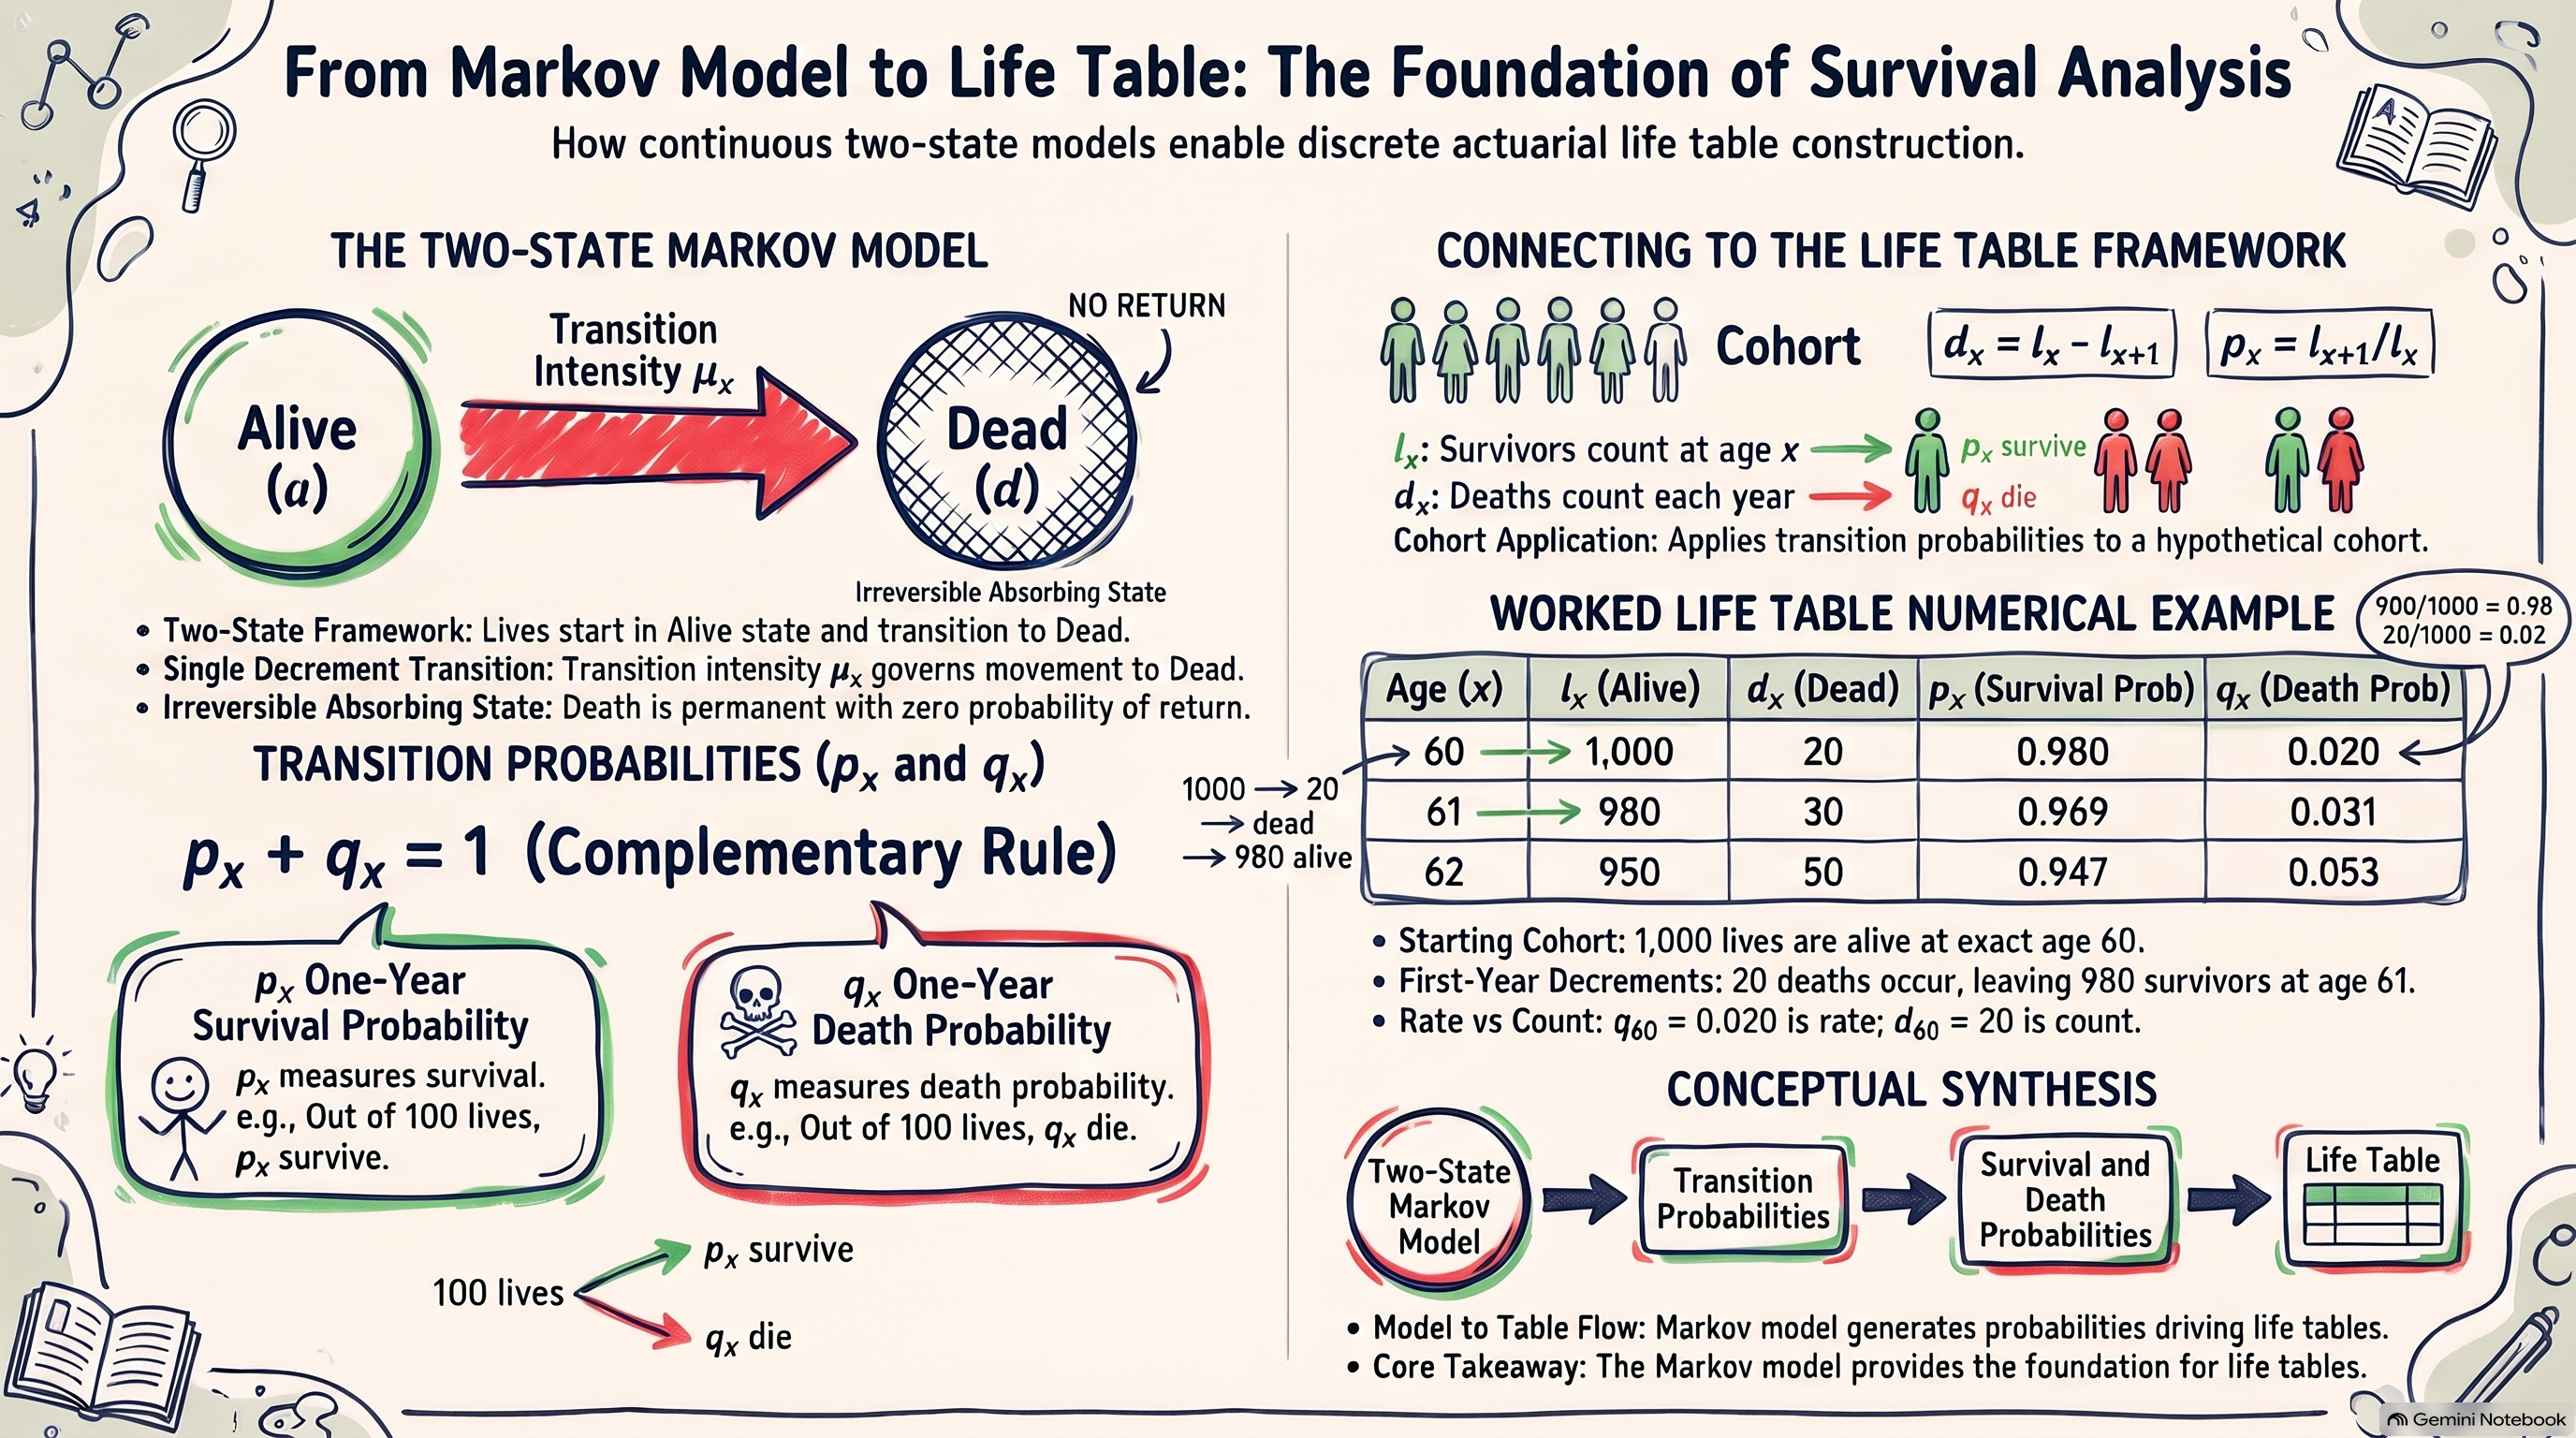
\includegraphics[width=0.75\linewidth,height=\textheight,keepaspectratio]{figures/Markov_Model_to_Life_Table.png}

}

\caption{Markov Model to Life Table}

\end{figure}%
\end{frame}

\section{The Two-State Markov Model}\label{the-two-state-markov-model}

\begin{frame}{The Two-State Model of a Single Decrement}
\protect\phantomsection\label{the-two-state-model-of-a-single-decrement}
The two-state Markov model describes the movement of an individual
between two states:

\begin{itemize}
\tightlist
\item
  State \(a\): Alive.
\item
  State \(d\): Dead.
\end{itemize}

The only possible transition is from Alive to Dead.

\begin{itemize}
\tightlist
\item
  Death is an irreversible transition.
\item
  The Dead state is an absorbing state.
\item
  The model is called a \textbf{single-decrement model} because there is
  only one possible type of transition out of the Alive state.
\end{itemize}
\end{frame}

\begin{frame}{Transition Diagram}
\protect\phantomsection\label{transition-diagram}
The movement between the two states can be represented by the following
transition diagram.

\[
\boxed{\text{Alive }(a)}
\quad\xrightarrow{\ \mu_x\ }\quad
\boxed{\text{Dead }(d)}
\]

Here, \(\mu_x\) denotes the transition intensity from Alive to Dead at
age \(x\).

The transition is one-way: an individual cannot return to the Alive
state after entering the Dead state.
\end{frame}

\begin{frame}{The Markov Property}
\protect\phantomsection\label{the-markov-property}
The Markov property states that the future development of the process
depends on its current state, rather than the sequence of states through
which it has passed.

For the two-state mortality model:

\begin{itemize}
\tightlist
\item
  If the individual is dead, they remain dead.
\item
  If the individual is alive, the possibility of death is described by
  the transition intensity at the current age.
\item
  The transition intensity may vary with the individual's attained age.
\end{itemize}

Thus, the model is a continuous-time Markov model in which the Dead
state is absorbing.
\end{frame}

\begin{frame}{Extension to Multiple States}
\protect\phantomsection\label{extension-to-multiple-states}
The two-state model provides a simple framework for modelling human
lifetime using the states Alive and Dead.

However, many actuarial problems involve more than two possible states.

For example, a life insurance model may distinguish between:

\begin{itemize}
\tightlist
\item
  \textbf{Healthy:} The individual is alive and in good health.
\item
  \textbf{Disabled:} The individual is alive but unable to work.
\item
  \textbf{Dead:} The individual has died.
\end{itemize}

Transitions may occur between these states, depending on the
individual's circumstances.

Such models are known as \textbf{multi-state models}. We will extend the
two-state framework to models with multiple states in the next chapter.
\end{frame}

\section{Transition Probabilities}\label{transition-probabilities}

\begin{frame}{Future Lifetime}
\protect\phantomsection\label{future-lifetime}
Let \(T_x\) denote the future lifetime of an individual currently aged
\(x\).

\begin{itemize}
\tightlist
\item
  \(T_x\) is a continuous random variable representing the remaining
  time until death.
\item
  Let \(w\) denote the \textbf{limiting age}, the maximum possible age
  of an individual.
\item
  In practice, the limiting age is often taken to be between 100 and 120
  years.
\end{itemize}

The age at death is therefore \(x+T_x\).
\end{frame}

\begin{frame}{Distribution and Survival Functions}
\protect\phantomsection\label{distribution-and-survival-functions}
The future lifetime \(T_x\) can be described using two functions.

\textbf{Distribution function}

\[
F_x(t)=P(T_x\leq t).
\]

This is the probability that an individual aged \(x\) dies within the
next \(t\) years.

\textbf{Survival function}

\[
S_x(t)=P(T_x>t).
\]

This is the probability that an individual aged \(x\) survives for more
than another \(t\) years.

Since \(T_x\) is continuously distributed, \(F_x(t)+S_x(t)=1.\)
\end{frame}

\begin{frame}{Actuarial Notation for Transition Probabilities}
\protect\phantomsection\label{actuarial-notation-for-transition-probabilities}
Actuaries use the following notation to describe the probabilities of
transitioning between the Alive and Dead states.

\textbf{Probability of death within \(t\) years:}

\[
{}_tq_x
= P(T_x\leq t)
= P(T_0\leq x+t\mid T_0>x).
\]

\textbf{Probability of survival for at least another \(t\) years:}

\[
{}_tp_x
= P(T_x>t)
= P(T_0>x+t\mid T_0>x).
\]

Here, \(T_0\) denotes the total lifetime from birth.

These probabilities satisfy

\[
{}_tp_x+{}_tq_x=1.
\]
\end{frame}

\begin{frame}{Definition of a Transition Probability}
\protect\phantomsection\label{definition-of-a-transition-probability}
The transition probability from one state to another is the probability
that an individual is in a particular state at a future time, given
their current state.

For the two-state model, the probability that a person aged \(x\) is
still alive at age \(x+t\) is

\[
{}_tp_x
=
P(\text{Alive at age }x+t
\mid
\text{Alive at age }x).
\]

Similarly, the probability that a person aged \(x\) is dead by age
\(x+t\) is

\[
{}_tq_x
=
P(\text{Dead by age }x+t
\mid
\text{Alive at age }x).
\]
\end{frame}

\begin{frame}{Transition Probability Matrix}
\protect\phantomsection\label{transition-probability-matrix}
The transition probabilities over an interval of length \(t\) can be
represented by a matrix.

Taking the state order as \((\text{Alive},\text{Dead})\),

\[
P_x(t)=
\begin{pmatrix}
{}_tp_x & {}_tq_x\\
0 & 1
\end{pmatrix}.
\]

\begin{itemize}
\tightlist
\item
  \({}_tp_x\): probability of remaining alive for another \(t\) years.
\item
  \({}_tq_x\): probability of moving from Alive to Dead within \(t\)
  years.
\item
  The Dead state is absorbing, so the individual remains dead with
  probability 1.
\end{itemize}
\end{frame}

\begin{frame}{Objective of the Two-State Markov Model}
\protect\phantomsection\label{objective-of-the-two-state-markov-model}
Our objective is to determine the transition probabilities between the
Alive and Dead states.

In particular, we would like to calculate

\[
{}_tp_x
=
P(\text{Alive at age }x+t
\mid
\text{Alive at age }x),
\]

the probability that a person currently aged \(x\) survives for at least
another \(t\) years.

Once we know this probability, we can also determine the probability of
death within \(t\) years using

\[
{}_tq_x=1-{}_tp_x.
\]

\textbf{The following sections develop the assumptions and methods
needed to calculate these transition probabilities.}
\end{frame}

\begin{frame}{Why Do We Need the Force of Mortality?}
\protect\phantomsection\label{why-do-we-need-the-force-of-mortality}
Suppose we compare two individuals, one aged 30 and the other aged 80.

Even if we know the probability that each individual dies within the
next year, these probabilities tell us only about the risk over that
particular year.

In actuarial modelling, we also want to understand how the risk of death
behaves at each age and how it changes as an individual gets older.

This motivates the need for a measure of the \textbf{instantaneous rate
of death}, which leads to the concept of the force of mortality.
\end{frame}

\begin{frame}{Force of Mortality}
\protect\phantomsection\label{force-of-mortality}
The probability of death over a short time interval depends on the
individual's current age.

The \textbf{force of mortality}, also called the transition intensity or
hazard rate, measures the instantaneous rate of death for an individual
who is alive at a given age.

At age \(x\), it is defined as

\[
\mu_x
=
\lim_{h\to 0^+}
\frac{1}{h}
P(T_0\leq x+h\mid T_0>x).
\]

Equivalently,

\[
\mu_x
=
\lim_{h\to 0^+}\frac{{}_hq_x}{h}.
\]

The force of mortality is measured per unit of time. Throughout this
chapter, we use years as the time unit.
\end{frame}

\begin{frame}{Transition Probabilities over a Short Interval}
\protect\phantomsection\label{transition-probabilities-over-a-short-interval}
For a sufficiently small time interval \(h\), the probability of death
can be approximated by

\[
{}_hq_x\approx \mu_x h.
\]

Similarly, the probability of remaining alive is approximately

\[
{}_hp_x\approx 1-\mu_xh.
\]

Thus, the probability of death over a short interval is approximately
proportional to:

\begin{itemize}
\tightlist
\item
  The length of the time interval, \(h\).
\item
  The force of mortality at the current age, \(\mu_x\).
\end{itemize}
\end{frame}

\begin{frame}{Worked Example: Short-Term Probability of Death}
\protect\phantomsection\label{worked-example-short-term-probability-of-death}
Suppose the force of mortality for a 70-year-old male in Thailand is
approximately

\[
\mu_{70}=0.05
\]

per year.

Calculate approximately the probability that he dies within:

\begin{enumerate}
\tightlist
\item
  One day.
\item
  One week.
\end{enumerate}
\end{frame}

\begin{frame}{Worked Example: Short-Term Probability of Death}
\protect\phantomsection\label{worked-example-short-term-probability-of-death-1}
\textbf{Solution}

For a short time interval \(h\), we use

\[
{}_hq_x\approx \mu_xh.
\]

\textbf{(a) Within one day}

Taking \(h=1/365\) years,

\[
\begin{aligned}
{}_{\frac{1}{365}}q_{70}
&\approx \frac{1}{365}\times 0.05\\
&\approx 0.000137.
\end{aligned}
\]

\textbf{(b) Within one week}

Taking \(h=7/365\) years,

\[
\begin{aligned}
{}_{\frac{7}{365}}q_{70}
&\approx \frac{7}{365}\times 0.05\\
&\approx 0.000959.
\end{aligned}
\]

The probability of death increases with the length of the observation
interval.
\end{frame}

\section{Assumptions Underlying the Markov
Model}\label{assumptions-underlying-the-markov-model}

\begin{frame}{The Markov Assumptions}
\protect\phantomsection\label{the-markov-assumptions}
The two-state Markov model is based on the following assumptions.

\begin{enumerate}
\item
  \textbf{Markov assumption:} The future state of an individual depends
  only on the current age and the state currently occupied, and not on
  the individual's previous history.
\item
  \textbf{Transition intensity assumption:} For a short time interval of
  length \(dt\), the probability of moving from Alive to Dead is

  \[
  {}_{dt}q_{x+t}
  =\mu_{x+t}\,dt+o(dt),
  \qquad t\geq 0.
  \]
\end{enumerate}

The second assumption states that the probability of death over a
sufficiently short interval is approximately proportional to the force
of mortality at the current age.

Here, \(o(dt)\) denotes a term that approaches zero faster than \(dt\)
as \(dt\to 0\), that is,

\[
\lim_{dt\to 0}\frac{o(dt)}{dt}=0.
\]
\end{frame}

\begin{frame}{An Equivalent Definition of the Transition Intensity}
\protect\phantomsection\label{an-equivalent-definition-of-the-transition-intensity}
The second assumption can also be expressed using a limit:

\[
\boxed{
\mu_{x+t}
=
\lim_{dt\to 0^+}
\frac{{}_{dt}q_{x+t}}{dt}
}
\]

This means that the force of mortality at age \(x+t\) is the
instantaneous rate of death for an individual who is alive at that age.

Thus, the transition intensity is the limiting probability of death per
unit of time over an increasingly short interval.
\end{frame}

\begin{frame}{Deriving the Survival Probability}
\protect\phantomsection\label{deriving-the-survival-probability}
We now derive the probability that an individual aged \(x\) survives for
at least another \(t\) years, denoted by \({}_tp_x\).

\textbf{Worked Example: Derivation of the Survival Probability}

Use the Markov assumptions to show that

\[
{}_tp_x
=
\exp\left(-\int_0^t\mu_{x+s}\,ds\right).
\]
\end{frame}

\begin{frame}{Deriving the Survival Probability}
\protect\phantomsection\label{deriving-the-survival-probability-1}
Consider the probability that an individual aged \(x\) survives to age
\(x+t+dt\).

By conditioning on the individual's state at age \(x+t\), we obtain

\[
\begin{aligned}
{}_{t+dt}p_x
&={}_tp_x\,{}_{dt}p_{x+t}
  +{}_tq_x\times 0\\
&={}_tp_x\,{}_{dt}p_{x+t}\\
&={}_tp_x\left(1-{}_{dt}q_{x+t}\right).
\end{aligned}
\]

The second term is zero because an individual who is dead at age \(x+t\)
cannot survive to age \(x+t+dt\).
\end{frame}

\begin{frame}{Applying the Transition Intensity Assumption}
\protect\phantomsection\label{applying-the-transition-intensity-assumption}
Recall the transition intensity assumption:

\[
{}_{dt}q_{x+t}
=\mu_{x+t}\,dt+o(dt).
\]

Substituting this into the survival probability gives

\[
\begin{aligned}
{}_{t+dt}p_x
&={}_tp_x\left(1-{}_{dt}q_{x+t}\right)\\
&={}_tp_x\left(1-\mu_{x+t}\,dt+o(dt)\right).
\end{aligned}
\]

Rearranging,

\[
\frac{{}_{t+dt}p_x-{}_tp_x}{dt}
=
-{}_tp_x\mu_{x+t}
+\frac{{}_tp_x\,o(dt)}{dt}.
\]
\end{frame}

\begin{frame}{Obtaining the Differential Equation}
\protect\phantomsection\label{obtaining-the-differential-equation}
Taking the limit as \(dt\to 0\), and using

\[
\lim_{dt\to 0}\frac{o(dt)}{dt}=0,
\]

we obtain

\[
\boxed{
\frac{d}{dt}{}_tp_x
=-\mu_{x+t}{}_tp_x.
}
\]

This differential equation describes how the survival probability
changes with time.

Since an individual aged \(x\) is alive at the starting time,
\(\boxed{{}_0p_x=1.}\)

This is the initial condition.
\end{frame}

\begin{frame}{Solving the Differential Equation}
\protect\phantomsection\label{solving-the-differential-equation}
We have the differential equation

\[
\frac{d}{dt}{}_tp_x
=-\mu_{x+t}{}_tp_x,
\qquad {}_0p_x=1.
\]

Separating the variables,

\[
\frac{d({}_tp_x)}{{}_tp_x}
=-\mu_{x+t}\,dt.
\]
\end{frame}

\begin{frame}{Solving the Differential Equation}
\protect\phantomsection\label{solving-the-differential-equation-1}
Integrating from \(0\) to \(t\),

\[
\begin{aligned}
\int_1^{{}_tp_x}\frac{1}{u}\,du
&=-\int_0^t\mu_{x+s}\,ds,\\
\ln({}_tp_x)
&=-\int_0^t\mu_{x+s}\,ds.
\end{aligned}
\]

Therefore, the survival probability is

\[
\boxed{
{}_tp_x
=
\exp\left(-\int_0^t\mu_{x+s}\,ds\right).
}
\]
\end{frame}

\begin{frame}{Constant Force of Mortality}
\protect\phantomsection\label{constant-force-of-mortality}
As a special case, suppose the force of mortality is constant over the
interval, so that

\[
\mu_{x+s}=\mu_x,
\qquad 0\leq s\leq t.
\]

Then the survival probability simplifies to

\[
\boxed{{}_tp_x=e^{-\mu_xt}.}
\]

Since \({}_tp_x+{}_tq_x=1\), the probability of death within \(t\) years
is

\[
\boxed{{}_tq_x=1-e^{-\mu_xt}.}
\]

Thus, under a constant force of mortality, the future lifetime \(T_x\)
follows an exponential distribution with parameter \(\mu_x\).
\end{frame}

\section{Estimation of the Force of
Mortality}\label{estimation-of-the-force-of-mortality}

\begin{frame}{Why Is Estimation Required?}
\protect\phantomsection\label{why-is-estimation-required}
The two-state Markov model describes the transition from Alive to Dead
through the force of mortality, \(\mu_x\).

\begin{itemize}
\tightlist
\item
  The force of mortality is generally unknown and must be estimated from
  observed mortality data.
\item
  Suppose we observe a sample of \(n\) independent lives over a
  specified age interval.
\item
  The observation period for each life may end either because the life
  dies or because the observation period ends.
\end{itemize}

The aim is to use these observations to estimate \(\mu_x\).
\end{frame}

\begin{frame}{Observing a Sample of Lives}
\protect\phantomsection\label{observing-a-sample-of-lives}
Suppose that \(n\) independent lives are observed at ages between \(x\)
and \(x+1\).

For life \(i\), where \(i=1,\ldots,n\), define:

\begin{itemize}
\tightlist
\item
  \(x+a_i\): age at which observation begins.
\item
  \(x+b_i\): planned age at which observation ends, provided the life
  survives.
\item
  \(x+t_i\): age at which observation actually ends, either through
  death or censoring.
\end{itemize}

Here, \(0\leq a_i\leq b_i<1\).

The actual observation period therefore begins at age \(x+a_i\) and ends
at age \(x+t_i\).
\end{frame}

\begin{frame}{Two Possible Observation Outcomes}
\protect\phantomsection\label{two-possible-observation-outcomes}
There are two possible outcomes for each observed life.

\textbf{Case 1: The life survives to the end of the observation period.}

\begin{itemize}
\tightlist
\item
  Observation ends at age \(x+b_i\).
\item
  The life is censored at the end of the observation period.
\item
  Hence, \(t_i=b_i\).
\end{itemize}

\textbf{Case 2: The life dies during the observation period.}

\begin{itemize}
\tightlist
\item
  Death occurs before age \(x+b_i\).
\item
  Observation ends at the age of death, \(x+t_i\).
\item
  Hence, \(t_i<b_i\).
\end{itemize}

The following diagrams illustrate these two cases.
\end{frame}

\begin{frame}{Censoring and Death Observation Outcomes}
\protect\phantomsection\label{censoring-and-death-observation-outcomes}
\begin{figure}[H]

{\centering 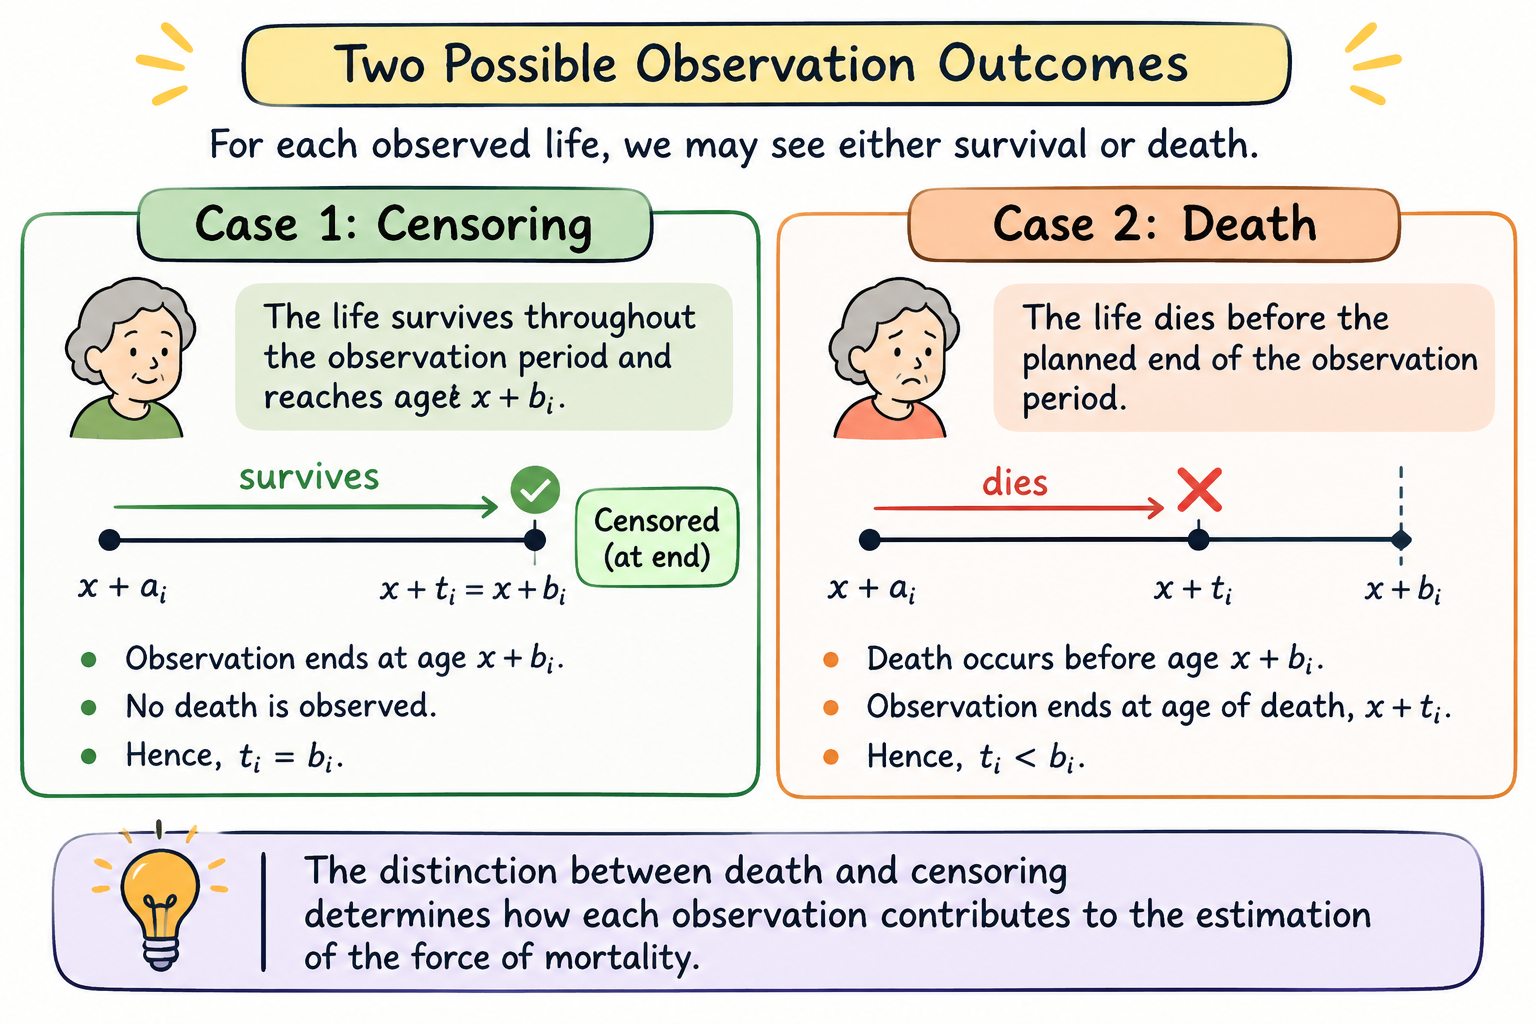
\includegraphics[width=0.75\linewidth,height=\textheight,keepaspectratio]{figures/Censoring_and_Death_Observation_Outcomes.png}

}

\caption{Censoring and Death Observation Outcomes}

\end{figure}%
\end{frame}

\begin{frame}{Case 1: Censoring}
\protect\phantomsection\label{case-1-censoring}
The life survives throughout the observation period and reaches age
\(x+b_i\).

\[
\text{Entry at } x+a_i \xrightarrow{\quad \text{Survival } (t_i) \quad} x+t_i = x+b_i \quad \color{red}{\text{(Censored)}}
\]

The observation ends without observing a death.
\end{frame}

\begin{frame}{Case 2: Death}
\protect\phantomsection\label{case-2-death}
The life dies before the planned end of the observation period.

\[
\text{Entry at } x+a_i \xrightarrow{\quad \text{Survival } (t_i) \quad} x+t_i < x+b_i \quad \color{red}{\text{(Death)}}
\]

The observation ends at the age of death.

The distinction between death and censoring determines how each
observation contributes to the estimation of the force of mortality.
\end{frame}

\begin{frame}{The Random Variables \(D_i\) and \(V_i\)}
\protect\phantomsection\label{the-random-variables-d_i-and-v_i}
The observations on life \(i\) can be described by two random variables:

\begin{itemize}
\tightlist
\item
  \(D_i\): an indicator of whether life \(i\) dies during the
  observation period.
\item
  \(V_i\): the observed waiting time from the beginning of observation
  until death or censoring.
\end{itemize}

Their observed values are denoted by \(d_i\) and \(v_i\), respectively.

Thus,

\[
D_i =
\begin{cases}
1, & \text{if life } i \text{ dies},\\
0, & \text{if life } i \text{ is censored},
\end{cases}
\]

and \(V_i=T_i-a_i,\)

where \(T_i\) denotes the observed stopping age measured relative to age
\(x\).

The estimation of the transition intensity \(\mu_x\) will be based on
the joint distribution of \(D_i\) and \(V_i\).
\end{frame}

\begin{frame}{Properties of \(D_i\) and \(V_i\)}
\protect\phantomsection\label{properties-of-d_i-and-v_i}
The random variables \(D_i\) and \(V_i\) have two important properties.

\textbf{1. They are dependent.}

The observed waiting time depends on whether the life dies or is
censored.

\begin{itemize}
\tightlist
\item
  If \(D_i=0\), the life survives to the end of the observation period,
  so that \(V_i=b_i-a_i\).
\item
  If \(D_i=1\), the life dies before the end of the observation period,
  so that \(V_i<b_i-a_i\).
\end{itemize}

\textbf{2. \(V_i\) has a mixed distribution.}

The distribution of \(V_i\) contains:

\begin{itemize}
\tightlist
\item
  A discrete probability mass at \(v_i=b_i-a_i\), corresponding to
  censoring.
\item
  A continuous probability density for \(0<v_i<b_i-a_i\), corresponding
  to death.
\end{itemize}

We derive these contributions under a simplifying assumption about the
force of mortality.
\end{frame}

\begin{frame}{Assumption: Constant Force of Mortality}
\protect\phantomsection\label{assumption-constant-force-of-mortality}
To derive the joint distribution of \(D_i\) and \(V_i\), assume that the
force of mortality is constant over the age interval \([x,x+1)\).

That is,

\[
\mu_{x+t}=\mu,
\qquad 0\leq t<1,
\]

where \(\mu\) is an unknown constant.

Under this assumption, the survival probability over an interval of
length \(v\) is

\[
{}_vp_{x+a_i}
=
\exp\left(-\int_0^v \mu\,ds\right)
=
e^{-\mu v}.
\]

We now derive the contribution to the joint distribution for each
possible observation outcome.
\end{frame}

\begin{frame}{Worked Example: Joint Distribution of \(D_i\) and \(V_i\)}
\protect\phantomsection\label{worked-example-joint-distribution-of-d_i-and-v_i}
Show that the contribution from the observation on life \(i\) can be
written as

\[
f_i(d_i,v_i)=e^{-\mu v_i}\mu^{d_i}.
\]

\textbf{Solution}

Let

\[
c_i=b_i-a_i
\]

denote the maximum possible observation period for life \(i\).

We consider the two possible cases:

\begin{enumerate}
\tightlist
\item
  \(D_i=0\): the life survives to the end of the observation period.
\item
  \(D_i=1\): the life dies during the observation period.
\end{enumerate}
\end{frame}

\begin{frame}{Case 1: The Life Is Censored (\(D_i=0\))}
\protect\phantomsection\label{case-1-the-life-is-censored-d_i0}
If life \(i\) survives to the end of the observation period, then

\[
V_i=b_i-a_i.
\]

The probability of observing this outcome is the probability that the
life survives from age \(x+a_i\) to age \(x+b_i\).

Hence,

\[
\begin{aligned}
&\Pr(D_i=0,V_i=b_i-a_i)\\
&\quad={}_{b_i-a_i}p_{x+a_i}\\
&\quad=\exp\left(
-\int_0^{b_i-a_i}\mu_{x+a_i+s}\,ds
\right).
\end{aligned}
\]
\end{frame}

\begin{frame}{Case 1: The Life Is Censored (\(D_i=0\))}
\protect\phantomsection\label{case-1-the-life-is-censored-d_i0-1}
Since the force of mortality is constant,

\[
\Pr(D_i=0,V_i=b_i-a_i)
=
e^{-\mu(b_i-a_i)}.
\]

As \(v_i=b_i-a_i\) in this case,

\[
\Pr(D_i=0,V_i=v_i)=e^{-\mu v_i}.
\]
\end{frame}

\begin{frame}{Case 1: Expressing the Contribution in a Common Form}
\protect\phantomsection\label{case-1-expressing-the-contribution-in-a-common-form}
Since \(D_i=0\), we have \(\mu^{D_i}=\mu^0=1\).

Therefore,

\[
\begin{aligned}
e^{-\mu v_i}
&=e^{-\mu v_i}\mu^0\\
&=e^{-\mu v_i}\mu^{D_i}.
\end{aligned}
\]

Thus, when life \(i\) is censored, its contribution is

\[
\boxed{e^{-\mu v_i}\mu^{D_i}}.
\]

We next consider the case in which life \(i\) dies during the
observation period.
\end{frame}

\begin{frame}{Case 2: The Life Dies (\(D_i=1\))}
\protect\phantomsection\label{case-2-the-life-dies-d_i1}
Suppose that life \(i\) dies at age \(x+a_i+v_i\), where

\[
0<v_i<b_i-a_i.
\]

For a small interval of length \(dv_i\), the probability that the life
survives for \(v_i\) years and then dies during the next interval of
length \(dv_i\) is

\[
\begin{aligned}
&\Pr(D_i=1,\ v_i\leq V_i<v_i+dv_i)\\
&={}_{v_i}p_{x+a_i}
\left(
\mu_{x+a_i+v_i}\,dv_i+o(dv_i)
\right).
\end{aligned}
\]

The first term is the probability of surviving up to the beginning of
the small interval. The second term is the probability of dying within
that interval, conditional on survival up to that point.
\end{frame}

\begin{frame}{Case 2: Deriving the Density}
\protect\phantomsection\label{case-2-deriving-the-density}
Under the constant force of mortality assumption,

\[
{}_{v_i}p_{x+a_i}=e^{-\mu v_i}
\]

and

\[
\mu_{x+a_i+v_i}=\mu.
\]

Therefore,

\[
\begin{aligned}
&\Pr(D_i=1,\ v_i\leq V_i<v_i+dv_i)\\
&=e^{-\mu v_i}
\left(\mu\,dv_i+o(dv_i)\right)\\
&=e^{-\mu v_i}\mu\,dv_i+o(dv_i).
\end{aligned}
\]
\end{frame}

\begin{frame}{Case 2: Deriving the Density}
\protect\phantomsection\label{case-2-deriving-the-density-1}
Dividing by \(dv_i\) and taking the limit as \(dv_i\to 0\) gives the
joint density contribution:

\[
\begin{aligned}
f_i(1,v_i)
&=\lim_{dv_i\to0}
\frac{
\Pr(D_i=1,\ v_i\leq V_i<v_i+dv_i)
}{dv_i}\\
&=e^{-\mu v_i}\mu.
\end{aligned}
\]
\end{frame}

\begin{frame}{Combining the Two Cases}
\protect\phantomsection\label{combining-the-two-cases}
We have obtained the following contributions:

{\def\LTcaptype{none} % do not increment counter
\begin{longtable}[]{@{}ll@{}}
\toprule\noalign{}
Observation outcome & Contribution \\
\midrule\noalign{}
\endhead
\(D_i=0\) (censored) & \(e^{-\mu v_i}\) \\
\(D_i=1\) (death) & \(\mu e^{-\mu v_i}\) \\
\bottomrule\noalign{}
\end{longtable}
}

Both cases can be expressed in a single form:

\[
\boxed{
f_i(d_i,v_i)
=
e^{-\mu v_i}\mu^{d_i}
}
\]

where \(d_i\in\{0,1\}\).

This expression gives the likelihood contribution from the observation
on life \(i\).

The next step is to combine the contributions from all \(n\) independent
lives to construct the likelihood function for estimating \(\mu\).
\end{frame}

\section{Maximum Likelihood
Estimation}\label{maximum-likelihood-estimation}

\begin{frame}{The Maximum Likelihood Estimate of \(\mu\)}
\protect\phantomsection\label{the-maximum-likelihood-estimate-of-mu}
Suppose that we observe \(n\) independent lives.

For life \(i\), we have:

\begin{itemize}
\tightlist
\item
  \(d_i\): an indicator of whether the life dies during the observation
  period.
\item
  \(v_i\): the observed waiting time, measured in years.
\end{itemize}

Recall that the likelihood contribution from life \(i\) is

\[
f_i(d_i,v_i)=e^{-\mu v_i}\mu^{d_i}.
\]

Since the \(n\) lives are independent, the likelihood function is
obtained by multiplying their individual contributions.
\end{frame}

\begin{frame}{Constructing the Likelihood Function}
\protect\phantomsection\label{constructing-the-likelihood-function}
Let

\[
\mathbf{d}=(d_1,d_2,\ldots,d_n)
\]

denote the observed death indicators, and let

\[
\mathbf{v}=(v_1,v_2,\ldots,v_n)
\]

denote the observed waiting times.

By independence, the total likelihood is proportional to

\[
\begin{aligned}
L(\mu;\mathbf{d},\mathbf{v})
&\propto \prod_{i=1}^{n}e^{-\mu v_i}\mu^{d_i}\\
&=e^{-\mu\sum_{i=1}^{n}v_i}
  \mu^{\sum_{i=1}^{n}d_i}.
\end{aligned}
\]
\end{frame}

\begin{frame}{Constructing the Likelihood Function}
\protect\phantomsection\label{constructing-the-likelihood-function-1}
Define the following summary statistics:

\begin{itemize}
\item
  Total observed waiting time: \[
  v=\sum_{i=1}^{n}v_i.
  \]
\item
  Total number of observed deaths: \[
  d=\sum_{i=1}^{n}d_i.
  \]
\end{itemize}

The likelihood function can therefore be written as

\[
\boxed{
L(\mu;d,v)\propto e^{-\mu v}\mu^d
}
\]
\end{frame}

\begin{frame}{Worked Example: Maximum Likelihood Estimation}
\protect\phantomsection\label{worked-example-maximum-likelihood-estimation}
Show that the maximum likelihood estimate of the constant force of
mortality \(\mu\) is

\[
\boxed{\hat{\mu}=\frac{d}{v}}.
\]
\end{frame}

\begin{frame}{Worked Example: Maximum Likelihood Estimation}
\protect\phantomsection\label{worked-example-maximum-likelihood-estimation-1}
\textbf{Solution}

From the previous result, the likelihood function is

\[
L(\mu;d,v)\propto e^{-\mu v}\mu^d.
\]

It is more convenient to maximise the log-likelihood function.

Taking logarithms gives

\[
\begin{aligned}
\ell(\mu)
&=\log L(\mu;d,v)\\
&=-\mu v+d\log\mu+C,
\end{aligned}
\]

where \(C\) is a constant that does not depend on \(\mu\).
\end{frame}

\begin{frame}{Differentiating the Log-Likelihood}
\protect\phantomsection\label{differentiating-the-log-likelihood}
To obtain the maximum likelihood estimate, differentiate the
log-likelihood with respect to \(\mu\):

\[
\frac{d\ell(\mu)}{d\mu}
=-v+\frac{d}{\mu}.
\]

Setting the first derivative equal to zero gives the likelihood
equation:

\[
-v+\frac{d}{\mu}=0.
\]

Rearranging, \(\frac{d}{\mu}=v.\)

Therefore, the maximum likelihood estimate is

\[
\boxed{
\hat{\mu}=\frac{d}{v}
}
\]
\end{frame}

\begin{frame}{Verifying the Maximum}
\protect\phantomsection\label{verifying-the-maximum}
The second derivative of the log-likelihood is

\[
\frac{d^2\ell(\mu)}{d\mu^2}
=-\frac{d}{\mu^2}.
\]

For \(d>0\) and \(\mu>0\),

\[
\frac{d^2\ell(\mu)}{d\mu^2}<0.
\]

Hence, the log-likelihood is strictly concave, and the stationary point
is the unique maximum.

Thus,

\[
\boxed{
\hat{\mu}=\frac{\text{Total number of observed deaths}}
{\text{Total observed waiting time}}
}
\]
\end{frame}

\begin{frame}{Actuarial Interpretation}
\protect\phantomsection\label{actuarial-interpretation}
The maximum likelihood estimate of the force of mortality is the ratio
of:

\begin{itemize}
\tightlist
\item
  The total number of observed deaths.
\item
  The total time for which lives were exposed to the risk of death.
\end{itemize}

Therefore,

\[
\boxed{
\text{Estimated force of mortality}
=
\frac{\text{Number of deaths}}
{\text{Total exposure to risk}}
}
\]

The total exposure to risk is measured in person-years.

For example, if 12 deaths are observed over a total exposure of 600
person-years, then

\[
\hat{\mu}=\frac{12}{600}=0.02.
\]

The estimated force of mortality is \(0.02\) per year, or 2 deaths per
100 person-years of exposure.
\end{frame}

\section{Statistical Properties and
Inference}\label{statistical-properties-and-inference}

\begin{frame}{Properties of the Maximum Likelihood Estimator}
\protect\phantomsection\label{properties-of-the-maximum-likelihood-estimator}
Recall that the maximum likelihood estimator of the constant force of
mortality is

\[
\tilde{\mu}=\frac{D}{V},
\]

where

\[
D=\sum_{i=1}^{n}D_i,
\qquad
V=\sum_{i=1}^{n}V_i.
\]

The observed estimate is \(\hat{\mu}=d/v\), where \(d\) and \(v\) are
the observed values of \(D\) and \(V\), respectively.

Let \(\mu_0\) denote the true (unknown) force of mortality.

By the Maximum Likelihood Theorem, the estimator \(\tilde{\mu}\) has the
following asymptotic properties as the sample size increases.
\end{frame}

\begin{frame}{Asymptotic Properties}
\protect\phantomsection\label{asymptotic-properties}
\textbf{1. Asymptotic unbiasedness}

The expected value of the estimator approaches the true force of
mortality:

\[
\boxed{
\mathrm{E}[\tilde{\mu}]
\longrightarrow \mu_0
}
\]

\textbf{2. Asymptotic efficiency}

The estimator achieves the Cramér--Rao lower bound asymptotically:

\[
\boxed{
\mathrm{Var}[\tilde{\mu}]
\approx I(\mu_0)^{-1}
}
\]

where \(I(\mu_0)\) is the Fisher information.
\end{frame}

\begin{frame}{Asymptotic Properties}
\protect\phantomsection\label{asymptotic-properties-1}
\textbf{3. Asymptotic normality}

For a sufficiently large sample,

\[
\boxed{
\tilde{\mu}
\approx
\mathcal{N}\left(
\mu_0,\frac{\mu_0}{\mathrm{E}[V]}
\right)
}
\]

Here, \(\mathrm{E}[V]\) denotes the expected total exposure over all
observed lives.
\end{frame}

\begin{frame}{Variance of the Estimator}
\protect\phantomsection\label{variance-of-the-estimator}
Under the constant force of mortality assumption, the expected number of
deaths and the expected total exposure satisfy

\[
\mathrm{E}[D]=\mu_0\mathrm{E}[V].
\]

The Fisher information is

\[
I(\mu_0)=\frac{\mathrm{E}[D]}{\mu_0^2}.
\]
\end{frame}

\begin{frame}{Variance of the Estimator}
\protect\phantomsection\label{variance-of-the-estimator-1}
Therefore,

\[
\begin{aligned}
I(\mu_0)^{-1}
&=\frac{\mu_0^2}{\mathrm{E}[D]}\\
&=\frac{\mu_0^2}{\mu_0\mathrm{E}[V]}\\
&=\frac{\mu_0}{\mathrm{E}[V]}.
\end{aligned}
\]

Hence, the asymptotic variance is

\[
\boxed{
\mathrm{Var}[\tilde{\mu}]
\approx
\frac{\mu_0}{\mathrm{E}[V]}
}
\]
\end{frame}

\begin{frame}{Estimating the Variance in Practice}
\protect\phantomsection\label{estimating-the-variance-in-practice}
Since the true force of mortality \(\mu_0\) is unknown, we replace it
with its maximum likelihood estimate:

\[
\hat{\mu}=\frac{d}{v}.
\]

We also use the observed total exposure \(v\) to estimate the expected
total exposure.

Thus,

\[
\begin{aligned}
\widehat{\mathrm{Var}}[\tilde{\mu}]
&\approx \frac{\hat{\mu}}{v}\\
&=\frac{d/v}{v}.
\end{aligned}
\]
\end{frame}

\begin{frame}{Estimating the Variance in Practice}
\protect\phantomsection\label{estimating-the-variance-in-practice-1}
Therefore,

\[
\boxed{
\widehat{\mathrm{Var}}[\tilde{\mu}]
=\frac{d}{v^2}
}
\]

The estimated standard error is

\[
\boxed{
\mathrm{SE}(\hat{\mu})
=\frac{\sqrt{d}}{v}
}
\]

This estimated standard error can be used to construct an approximate
confidence interval for the force of mortality.
\end{frame}

\begin{frame}{Confidence Interval for the Force of Mortality}
\protect\phantomsection\label{confidence-interval-for-the-force-of-mortality}
Using the asymptotic normality of the maximum likelihood estimator, an
approximate 95\% confidence interval for \(\mu_0\) is

\[
\boxed{
\hat{\mu}
\pm 1.96\,\mathrm{SE}(\hat{\mu})
}
\]

Equivalently,

\[
\boxed{
\left(
\hat{\mu}-1.96\frac{\sqrt{d}}{v},
\hat{\mu}+1.96\frac{\sqrt{d}}{v}
\right)
}
\]

Since the force of mortality must be positive, it is preferable to use a
confidence interval that respects this restriction.
\end{frame}

\begin{frame}{Confidence Interval for the Force of Mortality}
\protect\phantomsection\label{confidence-interval-for-the-force-of-mortality-1}
One approach is to construct an approximate confidence interval on the
logarithmic scale:

\[
\boxed{
\left(
\exp\left[\log\hat{\mu}
-1.96\frac{\mathrm{SE}(\hat{\mu})}{\hat{\mu}}\right],
\exp\left[\log\hat{\mu}
+1.96\frac{\mathrm{SE}(\hat{\mu})}{\hat{\mu}}\right]
\right)
}
\]

We illustrate these calculations using the following mortality data.
\end{frame}

\begin{frame}{Why Use the Logarithmic Scale?}
\protect\phantomsection\label{why-use-the-logarithmic-scale}
The force of mortality satisfies \(\mu>0\). However, an ordinary Wald
confidence interval may have a negative lower bound.

To construct an interval that respects this restriction, consider the
transformation

\[
g(\mu)=\log\mu.
\]

By the Delta Method,

\[
\begin{aligned}
\mathrm{SE}(\log\hat{\mu})
&\approx |g'(\hat{\mu})|\,
\mathrm{SE}(\hat{\mu})\\
&=\frac{\mathrm{SE}(\hat{\mu})}{\hat{\mu}}.
\end{aligned}
\]
\end{frame}

\begin{frame}{Why Use the Logarithmic Scale?}
\protect\phantomsection\label{why-use-the-logarithmic-scale-1}
Thus, an approximate 95\% confidence interval on the logarithmic scale
is

\[
\log\hat{\mu}
\pm 1.96\frac{\mathrm{SE}(\hat{\mu})}{\hat{\mu}}.
\]

Exponentiating the two endpoints gives a confidence interval for \(\mu\)
with strictly positive endpoints.
\end{frame}

\section{Applications of the Two-State Markov
Model}\label{applications-of-the-two-state-markov-model}

\begin{frame}{From Estimation to Application}
\protect\phantomsection\label{from-estimation-to-application}
So far, we have developed the two-state Markov model and shown how to
estimate the force of mortality from observed mortality data.

The model can now be used to estimate quantities of actuarial interest,
including:

\begin{itemize}
\tightlist
\item
  The force of mortality, \(\mu_x\).
\item
  The probability that a life aged \(x\) survives for a specified
  period.
\item
  The probability that a life aged \(x\) dies within a specified period.
\end{itemize}

In this section, we apply the model to observed mortality data and use
the estimated force of mortality to calculate transition probabilities.
\end{frame}

\begin{frame}{An Actuarial Application}
\protect\phantomsection\label{an-actuarial-application}
Consider an insurance company that observes a group of lives over a
specified age interval.

Some lives die during the observation period, while others survive to
the end of their observation periods.

Using the observed deaths and total exposure to risk, the company can:

\begin{enumerate}
\tightlist
\item
  Estimate the force of mortality.
\item
  Estimate the probability of death over a specified period.
\item
  Assess the mortality risk of the insured population.
\end{enumerate}

We illustrate these calculations using a sample of six observed lives.
\end{frame}

\begin{frame}{Worked Example: Mortality Data}
\protect\phantomsection\label{worked-example-mortality-data}
Consider the following mortality data for six independent lives, all
aged between \(x\) and \(x+1\).

{\def\LTcaptype{none} % do not increment counter
\begin{longtable}[]{@{}crrrr@{}}
\toprule\noalign{}
Life \(i\) & \(a_i\) & \(b_i\) & \(d_i\) & \(t_i\) \\
\midrule\noalign{}
\endhead
1 & 0 & 1 & 0 & 1 \\
2 & 0 & 1 & 1 & 0.5 \\
3 & 0 & 0.75 & 0 & 0.75 \\
4 & 0.25 & 0.75 & 1 & 0.5 \\
5 & 0.25 & 1 & 1 & 0.75 \\
6 & 0.5 & 1 & 0 & 1 \\
\bottomrule\noalign{}
\end{longtable}
}

Assume that the force of mortality \(\mu_x\) is constant over the age
interval \([x,x+1)\).
\end{frame}

\begin{frame}{Worked Example: Mortality Data}
\protect\phantomsection\label{worked-example-mortality-data-1}
Calculate:

\begin{enumerate}
\tightlist
\item
  The maximum likelihood estimate of \(\mu_x\).
\item
  The estimated variance of \(\tilde{\mu}\).
\item
  An approximate 95\% confidence interval for \(\mu_x\).
\item
  The estimated probability that a life aged \(x\) dies within one year.
\item
  The estimated variance of this probability.
\end{enumerate}
\end{frame}

\begin{frame}{Worked Example: Estimating the Force of Mortality}
\protect\phantomsection\label{worked-example-estimating-the-force-of-mortality}
Recall that

\[
\hat{\mu}=\frac{d}{v},
\]

where \(d\) is the total number of deaths and \(v\) is the total
observed exposure.
\end{frame}

\begin{frame}{Worked Example: Estimating the Force of Mortality}
\protect\phantomsection\label{worked-example-estimating-the-force-of-mortality-1}
First, calculate the observed waiting time for each life:

\[
v_i=t_i-a_i.
\]

{\def\LTcaptype{none} % do not increment counter
\begin{longtable}[]{@{}crr@{}}
\toprule\noalign{}
Life \(i\) & \(d_i\) & \(v_i=t_i-a_i\) \\
\midrule\noalign{}
\endhead
1 & 0 & 1 \\
2 & 1 & 0.5 \\
3 & 0 & 0.75 \\
4 & 1 & 0.25 \\
5 & 1 & 0.5 \\
6 & 0 & 0.5 \\
\textbf{Total} & \textbf{3} & \textbf{3.5} \\
\bottomrule\noalign{}
\end{longtable}
}
\end{frame}

\begin{frame}{Worked Example: Estimating the Force of Mortality}
\protect\phantomsection\label{worked-example-estimating-the-force-of-mortality-2}
Thus,

\[
d=\sum_{i=1}^{6}d_i=3, \quad \quad v=\sum_{i=1}^{6}v_i=3.5.
\]

The maximum likelihood estimate is

\[
\begin{aligned}
\hat{\mu}
&=\frac{d}{v} =\frac{3}{3.5} =0.85714.
\end{aligned}
\]

Therefore, the estimated force of mortality is

\[\boxed{\hat{\mu}=0.85714\text{ per year}.}\]
\end{frame}

\begin{frame}{Worked Example: Estimating the Variance}
\protect\phantomsection\label{worked-example-estimating-the-variance}
The estimated variance of \(\tilde{\mu}\) is

\[
\widehat{\mathrm{Var}}[\tilde{\mu}]
=\frac{d}{v^2}.
\]

Substituting \(d=3\) and \(v=3.5\) gives

\[
\begin{aligned}
\widehat{\mathrm{Var}}[\tilde{\mu}]
&=\frac{3}{3.5^2}\\
&=\frac{0.85714}{3.5}\\
&=0.24490.
\end{aligned}
\]
\end{frame}

\begin{frame}{Worked Example: Estimating the Variance}
\protect\phantomsection\label{worked-example-estimating-the-variance-1}
Hence,

\[
\boxed{
\widehat{\mathrm{Var}}[\tilde{\mu}]=0.24490
}
\]

The corresponding estimated standard error is

\[
\begin{aligned}
\mathrm{SE}(\hat{\mu})
&=\sqrt{0.24490}\\
&=0.49487.
\end{aligned}
\]
\end{frame}

\begin{frame}{Worked Example: 95\% Confidence Interval}
\protect\phantomsection\label{worked-example-95-confidence-interval}
Using the normal approximation, the 95\% Wald confidence interval is

\[
\hat{\mu}\pm1.96\sqrt{\widehat{\mathrm{Var}}[\tilde{\mu}]}.
\]

Substituting the estimated values gives

\[
\begin{aligned}
&0.85714\pm1.96\sqrt{0.24490}\\
&=(-0.11281,\ 1.82709).
\end{aligned}
\]
\end{frame}

\begin{frame}{Worked Example: 95\% Confidence Interval}
\protect\phantomsection\label{worked-example-95-confidence-interval-1}
However, the force of mortality must be positive.

We can instead construct an approximate confidence interval on the
logarithmic scale:

\[
\begin{aligned}
&\left(
\exp\left[\log(0.85714)
-1.96\frac{0.49487}{0.85714}\right],
\right.\\
&\qquad\left.
\exp\left[\log(0.85714)
+1.96\frac{0.49487}{0.85714}\right]
\right).
\end{aligned}
\]

Therefore, the approximate 95\% confidence interval is

\[
\boxed{(0.27644,\ 2.65769).}
\]
\end{frame}

\begin{frame}{Worked Example: Estimating the One-Year Death Probability}
\protect\phantomsection\label{worked-example-estimating-the-one-year-death-probability}
Under the two-state Markov model with a constant force of mortality,

\[
{}_tp_x=e^{-\mu_x t}.
\]

The probability that a life aged \(x\) dies within one year is

\[
q_x={}_1q_x=1-{}_1p_x.
\]

Therefore,

\[
q_x=1-e^{-\mu_x}.
\]
\end{frame}

\begin{frame}{Worked Example: Estimating the One-Year Death Probability}
\protect\phantomsection\label{worked-example-estimating-the-one-year-death-probability-1}
Replacing \(\mu_x\) with its maximum likelihood estimate gives

\[
\begin{aligned}
\hat{q}_x
&=1-e^{-\hat{\mu}}\\
&=1-e^{-0.85714}\\
&=0.57563.
\end{aligned}
\]

Hence,

\[
\boxed{\hat{q}_x=0.57563.}
\]

The estimated probability that a life aged \(x\) dies within one year is
approximately 57.56\%.
\end{frame}

\begin{frame}{Estimating the Variance of \(\hat{q}_x\)}
\protect\phantomsection\label{estimating-the-variance-of-hatq_x}
Since \(\hat{q}_x\) is a function of \(\hat{\mu}\), we can estimate its
variance using the \textbf{Delta Method}.

Suppose that \(X\) is an estimator of a parameter \(\theta\), with
variance \(\mathrm{Var}[X]\), and let \(g\) be a differentiable
function.

For a sufficiently large sample,

\[
\boxed{
\mathrm{Var}[g(X)]
\approx
[g'(\mathrm{E}[X])]^2\mathrm{Var}[X]
}
\]

In our application,

\[
g(\mu)=1-e^{-\mu}.
\]
\end{frame}

\begin{frame}{Estimating the Variance of \(\hat{q}_x\)}
\protect\phantomsection\label{estimating-the-variance-of-hatq_x-1}
Differentiating gives

\[
g'(\mu)=e^{-\mu}.
\]

Therefore, applying the Delta Method,

\[
\begin{aligned}
\mathrm{Var}[\hat{q}_x]
&\approx
\left(e^{-\hat{\mu}}\right)^2
\mathrm{Var}[\tilde{\mu}]\\
&=e^{-2\hat{\mu}}
\mathrm{Var}[\tilde{\mu}].
\end{aligned}
\]
\end{frame}

\begin{frame}{Worked Example: Variance of the One-Year Death
Probability}
\protect\phantomsection\label{worked-example-variance-of-the-one-year-death-probability}
Substituting the estimated force of mortality and its variance gives

\[
\begin{aligned}
\widehat{\mathrm{Var}}[\hat{q}_x]
&\approx e^{-2(0.85714)}(0.24490)\\
&=0.04410.
\end{aligned}
\]

Thus,

\[
\boxed{
\widehat{\mathrm{Var}}[\hat{q}_x]
\approx 0.04410
}
\]

The estimated standard error of \(\hat{q}_x\) is

\[
\mathrm{SE}(\hat{q}_x)
=\sqrt{0.04410}
\approx 0.21001.
\]

The variance of the estimated one-year death probability is obtained
from the variance of the estimated force of mortality using the Delta
Method.
\end{frame}

\begin{frame}{Summary of the Worked Example}
\protect\phantomsection\label{summary-of-the-worked-example}
For the six observed lives, we obtain the following results.

{\def\LTcaptype{none} % do not increment counter
\begin{longtable}[]{@{}lr@{}}
\toprule\noalign{}
Quantity & Estimate \\
\midrule\noalign{}
\endhead
Total number of deaths, \(d\) & 3 \\
Total exposure, \(v\) & 3.5 person-years \\
Force of mortality, \(\hat{\mu}\) & 0.85714 \\
Estimated variance of \(\tilde{\mu}\) & 0.24490 \\
Estimated standard error of \(\hat{\mu}\) & 0.49487 \\
One-year death probability, \(\hat{q}_x\) & 0.57563 \\
Estimated variance of \(\hat{q}_x\) & 0.04410 \\
\bottomrule\noalign{}
\end{longtable}
}

The two-state Markov model therefore provides a way to estimate both the
force of mortality and the corresponding transition probabilities from
observed mortality data.
\end{frame}

\begin{frame}{Worked Example 1: Survival Probabilities}
\protect\phantomsection\label{worked-example-1-survival-probabilities}
An insurance company models the mortality of a group of lives aged 60
using a two-state Markov model. The force of mortality is assumed to be
constant at 0.025 per annum.

Calculate:

\begin{enumerate}
\tightlist
\item
  The probability that a life aged 60 survives for five years.
\item
  The probability that the life dies within the next three years.
\item
  The probability that a life aged 60 survives for eight years, given
  that the life has already survived for five years.
\item
  Calculate the probability that a life aged 60 survives for five years
  and then dies within the following three years.
\end{enumerate}
\end{frame}

\begin{frame}{Solution: Worked Example 1}
\protect\phantomsection\label{solution-worked-example-1}
\end{frame}

\begin{frame}{Worked Example 2: Piecewise Constant Force of Mortality}
\protect\phantomsection\label{worked-example-2-piecewise-constant-force-of-mortality}
A life aged 50 is subject to the following forces of mortality:

\[
\mu_{50+t}=
\begin{cases}
0.01, & 0\leq t<5,\\
0.02, & 5\leq t<10.
\end{cases}
\]

Calculate:

\begin{enumerate}
\tightlist
\item
  The probability that the life survives to age 55.
\item
  The probability that the life survives to age 60.
\item
  The probability that the life dies between ages 55 and 60.
\item
  The probability that the life survives for another three years, given
  that the life is currently aged 57.
\end{enumerate}
\end{frame}

\begin{frame}{Solution: Worked Example 2}
\protect\phantomsection\label{solution-worked-example-2}
\end{frame}

\begin{frame}{Worked Example 3: Estimating the Force of Mortality}
\protect\phantomsection\label{worked-example-3-estimating-the-force-of-mortality}
A life office observes the following life-table values:

{\def\LTcaptype{none} % do not increment counter
\begin{longtable}[]{@{}lr@{}}
\toprule\noalign{}
Age & Number alive \\
\midrule\noalign{}
\endhead
65 & 10,000 \\
66 & 9,850 \\
67 & 9,700 \\
\bottomrule\noalign{}
\end{longtable}
}

Assume that the force of mortality is constant within each year of age.

Calculate:

\begin{enumerate}
\tightlist
\item
  The estimated force of mortality between ages 65 and 66.
\item
  The estimated force of mortality between ages 66 and 67.
\item
  The corresponding one-year probabilities of death.
\item
  The probability that a life aged 65 survives to age 67.
\end{enumerate}
\end{frame}

\begin{frame}{Solution: Worked Example 3}
\protect\phantomsection\label{solution-worked-example-3}
\end{frame}

\begin{frame}{Worked Example 4: Number of Deaths in a Portfolio}
\protect\phantomsection\label{worked-example-4-number-of-deaths-in-a-portfolio}
An insurance company observes a portfolio of 500 independent lives, all
aged 70, over a one-year period.

Assume that each life is subject to a constant force of mortality of
0.02 per annum.

Calculate:

\begin{enumerate}
\tightlist
\item
  The probability that an individual life dies during the year.
\item
  The expected number of deaths during the year.
\item
  The approximate probability that at least 12 deaths occur during the
  year, using a Poisson approximation.
\item
  The probability that no more than 8 deaths occur during the year,
  using a Poisson approximation.
\end{enumerate}
\end{frame}

\begin{frame}{Solution: Worked Example 4}
\protect\phantomsection\label{solution-worked-example-4}
\end{frame}

\begin{frame}{Worked Example 5: Maximum Likelihood Estimation of the
Force of Mortality}
\protect\phantomsection\label{worked-example-5-maximum-likelihood-estimation-of-the-force-of-mortality}
An insurance company observes 200 independent lives, all aged 75, over a
period of one year. During this period, 12 lives die and the remaining
lives survive to the end of the observation period.

Assume that all lives are subject to the same constant force of
mortality, \(\mu\).

Calculate:

\begin{enumerate}
\tightlist
\item
  The likelihood function for \(\mu\).
\item
  The maximum likelihood estimator of \(\mu\).
\item
  The estimated probability that a life aged 75 survives for two years.
\item
  The estimated probability that a life aged 75 dies within the next six
  months.
\end{enumerate}
\end{frame}

\begin{frame}{Solution: Worked Example 5}
\protect\phantomsection\label{solution-worked-example-5}
\end{frame}

\section{Further Remarks}\label{further-remarks}

\begin{frame}{Relationship Between Life Table Functions and the Force of
Mortality}
\protect\phantomsection\label{relationship-between-life-table-functions-and-the-force-of-mortality}
A life table typically contains discrete mortality measures, such as:

\begin{itemize}
\tightlist
\item
  \(l_x\): number of lives surviving to exact age \(x\).
\item
  \(d_x\): number of deaths between ages \(x\) and \(x+1\).
\item
  \(q_x\): probability of death between ages \(x\) and \(x+1\).
\item
  \(p_x\): probability of survival from age \(x\) to age \(x+1\).
\end{itemize}

These quantities are related by

\[
q_x=\frac{d_x}{l_x},
\qquad
p_x=1-q_x=\frac{l_{x+1}}{l_x}.
\]

A life table may also include the force of mortality, \(\mu_x\), which
describes the instantaneous rate of mortality at exact age \(x\). More
generally, \(\mu_{x+t}\) denotes the force of mortality at age \(x+t\),
where \(0\leq t\leq 1\).
\end{frame}

\begin{frame}{Relationship between the force of mortality and survival
probability}
\protect\phantomsection\label{relationship-between-the-force-of-mortality-and-survival-probability}
The probability that a life aged \(x\) survives for \(t\) years is

\[
{}_tp_x
=
\exp\left(-\int_0^t\mu_{x+s}\,ds\right).
\]

In particular, the one-year survival probability is

\[
p_x
=
\exp\left(-\int_0^1\mu_{x+s}\,ds\right).
\]

The life table provides the one-year survival probability, but it does
not specify how the force of mortality varies within the year.
\end{frame}

\begin{frame}{Relationship Between Life Table Functions and the Force of
Mortality}
\protect\phantomsection\label{relationship-between-life-table-functions-and-the-force-of-mortality-1}
For example, between ages 20 and 21, the force of mortality may vary at
different ages, such as:

\begin{itemize}
\tightlist
\item
  \(\mu_{20}\): force of mortality at exact age 20.
\item
  \(\mu_{20+1/12}\): force of mortality at age 20 years and 1 month.
\item
  \(\mu_{20+6/12}\): force of mortality at age 20 years and 6 months.
\item
  \(\mu_{20+11/12}\): force of mortality at age 20 years and 11 months.
\end{itemize}

Thus, knowing \(p_{20}\) alone does not determine the instantaneous
force of mortality at every age between 20 and 21.
\end{frame}

\begin{frame}{Constant force of mortality assumption}
\protect\phantomsection\label{constant-force-of-mortality-assumption}
If we assume that the force of mortality is constant between ages \(x\)
and \(x+1\), then

\[
\mu_{x+t}=\mu_x,
\qquad 0\leq t\leq 1.
\]

The relationship between the one-year survival probability and the force
of mortality becomes

\[
p_x=e^{-\mu_x}.
\]

Therefore,

\[
\boxed{\mu_x=-\ln(p_x).}
\]
\end{frame}

\begin{frame}{Constant force of mortality assumption}
\protect\phantomsection\label{constant-force-of-mortality-assumption-1}
Since

\[
p_x=\frac{l_{x+1}}{l_x}
=1-\frac{d_x}{l_x},
\]

we can also calculate the force of mortality directly from the life
table:

\[
\boxed{
\mu_x
=-\ln\left(\frac{l_{x+1}}{l_x}\right)
=-\ln\left(1-\frac{d_x}{l_x}\right).
}
\]

Both expressions give the same result.
\end{frame}

\begin{frame}{Key distinction}
\protect\phantomsection\label{key-distinction}
\begin{itemize}
\tightlist
\item
  Without an additional assumption, the life table determines the
  integrated force of mortality over the year:
\end{itemize}

\[
\int_0^1\mu_{x+t}\,dt=-\ln(p_x).
\]

\begin{itemize}
\tightlist
\item
  Under the constant force of mortality assumption, we can calculate the
  instantaneous force of mortality directly:
\end{itemize}

\[
\mu_x=-\ln(p_x).
\]

Therefore, \(l_x\) and \(d_x\) can be used to calculate \(\mu_x\), but
this requires the assumption that the force of mortality is constant
over the year of age.
\end{frame}




\end{document}
